\chapter{First steps towards the station calibration}\label{planning}
\textit{Following the comprehensive testing of the DAQ and FEE, the subsequent crucial 
step towards achieving a fully operational tracker is the calibration phase. This 
calibration will be carried out exploiting cosmic muons. The primary objective of 
this calibration process is to accurately determine signal propagation times and 
channel-to-channel delays within each straw. To accomplish this, it is essential 
to perform an unbiased reconstruction of the longitudinal position of the hits 
within the straws. This would be easily achieved using the station orientated horizontally. 
However, certain technical and mechanical contingencies prevent horizontal calibration, 
necessitating the exclusive focus on vertical orientation.
This Chapter focuses on reconstructing the trajectories of cosmic muons within a vertically oriented 
station, as well as analyzing potential biases and systematic errors that could 
arise from this particular orientation.}
\section{Overview of the timing calibration}
When a charged particle crosses the straw tube 
gas volume, the resulting ionization charge 
generates an electric signal along the anode  
wire which propagates towards the two ends of 
the straw and to the front-end electronics, 
where TDCs measure the signal arrival 
times $t_1$ and $t_2$. The primary goal of 
the timing calibration is to enable the 
determination of the track position 
along the straw from the measurement of 
the arrival times $t_1$ and $t_2$. 
The dependence of $t_1$ and $t_2$ on the track 
position $x_{\text{track}}$ is given by the following equations:
\begin{equation}
\begin{aligned}
    t_1 &= t_0 + \frac{x_{\text{track}}}{v} + t_d + d_1 \\
    t_2 &= t_0 + \frac{L - x_{\text{track}}}{v} + t_d + d_2
\end{aligned}
\end{equation}
where $t_0$ is the particle's crossing time, 
$t_d$ is the drift time in the straw, 
$L$ is the length of the straw, 
$x_{\text{track}}$ is the 
reconstructed track position on the wire, $v$ 
is the propagation velocity of 
the electric signal along the anode 
wire and $d_i$ are the delays  
introduced by the front end electronics. 
$t_1$ and $t_2$ are measured  
by the TDCs on the front-end HV side and on the CAL side.
The measurement of the time difference 
$\Delta t_{12}=t_1-t_2$ allows 
determining the coordinate $x_{\text{track}}$, 
while $(t_1 + t_2) / 2$ allows to measure the drift time  
up to an offset common to all channels. 
If we subtract and add the two equations:
\begin{equation}\label{ffffff}
    \begin{aligned}
        \Delta t_{12} &= \frac{2x_{\text{track}}-L}{v} +(d_1-d_2)  \\
        \frac{(t_1 + t_2)}{2} &= t_d+t_0+\frac{d_1+d_2}{2}-\cfrac{L}{2v} 
    \end{aligned}
    \end{equation}
The first equation contains the time 
difference $\Delta t_{12}$ between the 
signals at the two straw ends as measured 
by the TDCs, the reconstructed track coordinate 
$x_{\text{track}}$ along the wire, the propagation  
velocity $v$ of the signal along the wire and 
the difference $d_1-d_2$ between the delays introduced by 
the front-end electronics. 
Performing the timing calibration means 
determining $v$ and $d_1-d_2$ from the $\Delta t_{12}$ 
measured by the TDCs and from an independent and unbiased 
reconstruction of the track 
projected on the wire ($x_{\text{track}}$).
This is the first calibration of the detector and 
will be performed using cosmic muons. 
At this level, the only available spatial 
information is whether a straw has been crossed 
by a muon or not. The 
only way to obtain $x_{\text{track}}$ from a "yes or no" 
information is to rely on the tracker station 
geometry (Section \ref{reconstruction}).


\subsection{Operational constraints of the station}\label{gassystem}
The detector, its infrastructures 
and services, and, consequently, the stations have been
designed for being operated in a 
$vertical$ $orientation$. This has now an impact 
on several aspects of detection operation: from 
the storage and handling tools of the fully assembled and 
equipped station, which is a very fragile system, to
the available services, for example the gas 
distribution system, which have been designed for
managing, moving and operating a complex 
detector with a specific orientation, and may not
allow to move and operate even one single 
station, in a different orientation. 
The most reasonable orientation of the station for a test with
cosmic muons is the $horizontal$ $orientation$. 
That facilitates unbiased 
reconstruction, since cosmic muons are distributed according to 
cos$^2\theta$ and they are predominantly vertical 
(Section \ref{distcos}), thus crossing the straws mostly perpendicularly.
Initially, the operational constraints, which may prevent the station from being operated horizontally, were assessed.
Apparently, the main challenge with the horizontal orientation is the operation of the gas
distribution system. The gas distribution system of the panel is equipped with two check valves:
the first one is located on the supply side, the second one on the exhaust side. These valves
operate using a simple mechanism where a ball is pressed onto an O-ring to form a seal. The
only operational mode for these valves is to be oriented vertically to ensure proper sealing. In
our specific case, this is not an issue for the check valves on the supply side, since they should
be kept open during calibration to allow gas flowing. On the other hand, the check valves on
the exhaust side of the panel must be closed at all times to prevent gas from leaking before
reaching the panel. Figure \ref{fig:gassystem} shows a schematic 
representation of the operational mode of the supply 
and exhaust valves. The red arrows represent the 
direction of the gas flow. On the supply side (Figure 
\ref{fig:gassystem} (Left)), the ball has to rest on the 
O-ring, or the gas flows downwards towards the atmosphere, 
rather than flowing upwards towards the panel. According 
to these specifications, it seems that the only operational 
mode of the station is in the vertical position. 
Additionally, other reasons include space constraints, as placing 
a station horizontally takes significantly more space than 
vertically. Moreover, the station is quite fragile, and 
excessive movement could lead to potential issues.

The ultimate goal is to perform a timing calibration of 
the first assembled station of the tracker using 
cosmic muons, with the aim of achieving a longitudinal hit 
position resolution better than 4 cm. This would enable a better distinction 
between different particle trajectories while reconstructing helices (Appendix \ref{eventreco}).

In the following section, simulation performed to reconstruct cosmic tracks will be described with  
a vertically oriented station, with the aim of understanding 
potential biases in determining the longitudinal position.

\begin{figure}[!h]
    \centering
    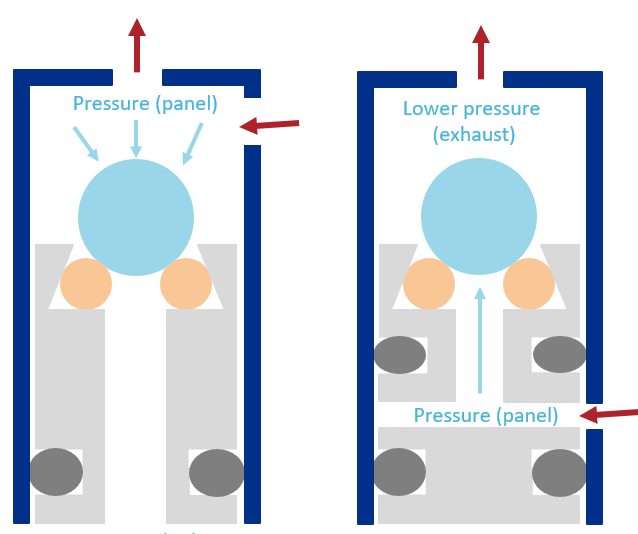
\includegraphics[width =0.4\textwidth]{figures/png/gassystem.png}
    \caption[Schematic view of the valves located in a tracker panel.]{Schematic view of the valves located in a tracker panel.}
    \label{fig:gassystem}
\end{figure}
To ensure optimal performance, it is essential to take data with a vertical oriented station 
to achieve conditions that are as close as possible to those of the real detector. 
However, if the vertical orientation proves ineffective for calibration, 
alternative mechanical solutions will be considered.

This Chapter reports on a simulation study 
which shows that the vertical orientation introduces a significant bias on 
the $x_{\text{track}}$ which significantly complicates 
the station calibration. 



\section{Cosmic muons as a calibration source}
Cosmic muons will play a fundamental role in the 
calibration of the entire Mu2e detector system and, 
in particular, the tracker. They have unique 
characteristics that make calibration with cosmic rays 
complementary to other techniques:

 

\begin{itemize}
    \item calibration samples with cosmic muons 
    can be taken during standard detector operations, 
    with the same detector conditions as the physics samples;
    \item the cosmic muons flux 
    ($\sim 1 \ \text{cm}^{-2} \text{min}^{-1}$ 
    for horizontal detectors and a mean
    muon energy of $\sim$4 GeV \cite{muonflux}) 
    is sufficient to allow
    collecting a substantial amount of calibration 
    data in a relatively short time and 
    thus monitoring continuously the detector response;
    \item a cosmic muon is a minimum ionizing 
    particle (MIP) and 
    its energy loss is almost 
    independent of its energy;
    \item the speed of the cosmic muons is equal to the 
    speed of light $c$, and the time they take to traverse 
    a detector, in our case one tracker station, can be 
    used to align the time offsets of all the channels  
    without any external time reference.
\end{itemize}
\subsection{Cosmic muons energy and angular distribution}\label{distcos}
The muon flux at sea level is usually described by the Gaisser formula \cite{guan2015parametrization}:
\begin{equation}
    \frac{d I}{d E_\mu d \Omega d t d S}=\frac{0.14}{\mathrm{~cm}^2 \mathrm{~s} \ \mathrm{sr}}\left(\frac{E_\mu}{\mathrm{GeV}}\right)^{-2.7} \quad\left[\frac{1}{1+\frac{1.1 E_\mu \cos \theta}{115 \mathrm{GeV}}}+\frac{0.054}{1+\frac{1.1 E_\mu \cos \theta}{850 \mathrm{GeV}}}\right]
    \end{equation}
where $E_\mu$ is the muon energy and $\theta$ is the muon polar angle. 
The two terms in brackets correspond to the contribution of the charged pions and kaons, while 
the small contribution from charm and heavier flavors is neglected. 
This simplified formula doesn't take into account muon decays and the curvature of the Earth, 
thus it is only valid for zenith angles $\theta < 70^\circ$
and for energies $E > \frac{100}{\cos \theta}$ GeV.

A modified version of the standard Gaisser formula, called Gaisser-Tang model, is used to account for low energy and large zenith angle effects \cite{guan2015parametrization}:
\begin{equation}\label{cosmicmuonflux}
    \frac{d I}{d E_\mu d \Omega d t d S}=\frac{0.14}{\mathrm{cm}^2 \mathrm{~s} \ \mathrm{sr} }\left( \frac{E_\mu}{\mathrm{GeV}} \left(1+\frac{3.64 \mathrm{GeV}}{E_\mu\left(\cos \theta^*\right)^{1.29}}\right)\right)^{-2.7}\left[\frac{1}{1+\frac{1.1 E_\mu \cos \theta^*}{115 \mathrm{GeV}}}+\frac{0.054}{1+\frac{1.1 E_\mu \cos \theta^*}{850 \mathrm{GeV}}}\right]
\end{equation}
where the second term in the bracket is the same as in the standard formula, except that the zenith angle 
$\theta$ is substituted by the angle $\theta^*$. The relation between cos$\theta$
and cos$\theta^*$ is given by:
\begin{equation}
    \cos \theta^*=\sqrt{\frac{(\cos \theta)^2+P_1^2+P_2(\cos \theta)^{P_3}+P_4(\cos \theta)^{P_5}}{1+P_1^2+P_2+P_4}}
    \end{equation}
The parameters $P_1$ = 0.102573, $P_2$ = -0.068287, $P_3$ = 0.958633, $P_4$ = 0.0407253, and $P_5$ = 0.817285 were calculated using 
a dedicated simulation of muon production in the atmosphere. A representation of the angles is shown in Figure \ref{fig:anglesinmuon}.
Another factor is included in Equation \ref{cosmicmuonflux} to account for the possibility of muon decays, which are more 
significant at low energies. The numerical constants are derived by fitting experimental data from various cosmic muon studies.
\begin{figure}[!h]
    \centering
    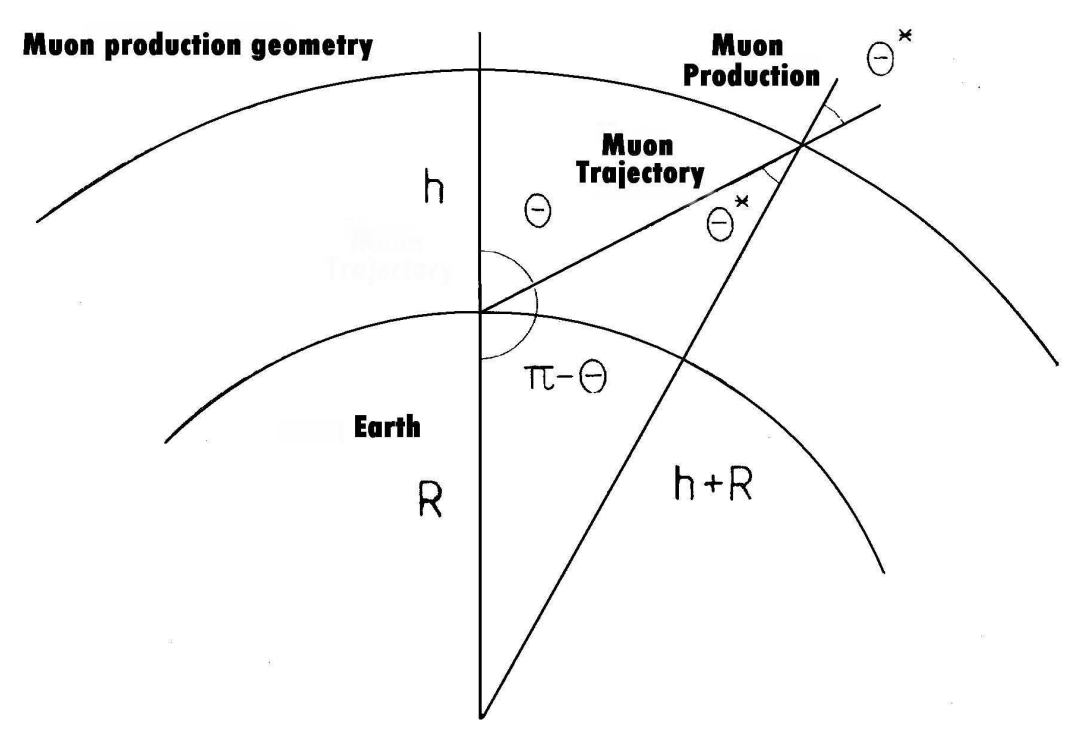
\includegraphics[width =0.6\textwidth]{figures/png/Screenshot_20240526_140716.png}
    \caption[The relation of $\theta^*$ to $\theta$.]{The relation of the observed zenith angle of muons, $\theta^*$, to 
    the zenith angle at the muon production point in the atmosphere, $\theta$. 
    $R$ is the radius of the Earth \cite{guan2015parametrization}.}
    \label{fig:anglesinmuon}
\end{figure}

\subsection{Monte Carlo cosmic generation with CRY}
Several Monte Carlo programs allow to simulate sea-level 
cosmic ray muons: the most widely used is CRY, developed 
by Los Alamos National Laboratory (LANL). CRY \cite{Hagmann2007CosmicraySG} functions as a generator for air showers 
induced by primary cosmic rays. The CRY package uses 
precomputed input tables derived from comprehensive 
MCNPX 2.5.0 simulation of protons in the energy range 
between 1 GeV and 100 TeV, at the top of the atmosphere.
The generation of muons and other secondary particles 
is governed by the pion and kaon decays. The package 
generates the cosmic muon flux within a zenith angle range 
of 0-90°, following a cos$^2 \theta$ distribution, and an 
energy range between 1-100 GeV, following the Gaisser-Tang
parameterization.The CRY package accounts for the 
dependence of cosmic muon flux on various parameters, 
including altitude, latitude, and solar activity. CRY 
provides muon flux data at three different altitudes: 
sea level, 2100 m, and 11300 m, with sea level being 
selected for this study. The latitude is set at 41.8° N, 
corresponding to Fermilab. To avoid variations of the 
primary cosmic muon flux due to solar activity, a 
common day (6-21-2021) was chosen outside the maximum and minimum 
sunspot cycle for the simulation. While there are other 
packages designed to produce cosmic muons with specific 
energy and zenith angles, such as CORSIKA \cite{Heck:1998vt}, CRY was chosen 
for its straightforward implementation.


\subsection{Monte Carlo sample and coordinate system }\label{genplane}
A sample of cosmic muons was generated with a uniform distribution within a
horizontal plane approximately 11 m above the muon beam axis. The GEANT4 
simulation also incorporates the effects of the external neutron shield surrounding the DS 
and the concrete ceiling of the Mu2e experimental hall. Starting from the generation plane, 
cosmic muons pass through the concrete ceiling and walls situated outside the experimental hall. 
As they propagate downwards to the detector, they interact with the building materials. 
The external neutron shield surrounding the DS consists of concrete ($\rho$=2.3 g/cm$^3$) of  
roughly 0.9 m thickness, while the ceiling above the Mu2e experimental area comprises 1.8 m of concrete. 
The entire structure is enclosed within a volume of air at standard temperature and pressure.

The simulation of the station was performed in what in Mu2e jargon is called
"extracted position", which means the station was placed outside the solenoid.
Given that the Earth's magnetic field is approximately 
$4 \div 5 \times 10^{-5}$ T, 
and considering that the dimensions of the station are 
on the order of 1-2 m, 
along with the fact that the majority of particles under consideration
have energies around $\sim$ 1 GeV, 
the curvature radius of the particles is approximately 
$R\sim p[\text{GeV}]/(B[\text{T}]\cdot 0.3) \sim 70$ km. 
This radius is significantly larger than the station's 
dimensions, allowing us to reconstruct particle trajectories 
as straight lines.
For this reason, in the simulation  
the magnetic field was set to zero. 

Before describing the event selection and the 
reconstruction, it is important to define the coordinate system, 
as shown in Figure \ref{fig:coordinate}. The $z$ axis is parallel to 
the DS axis, while the $y$ axis corresponds to the vertical axis.
\begin{figure}[!h]
    \centering
    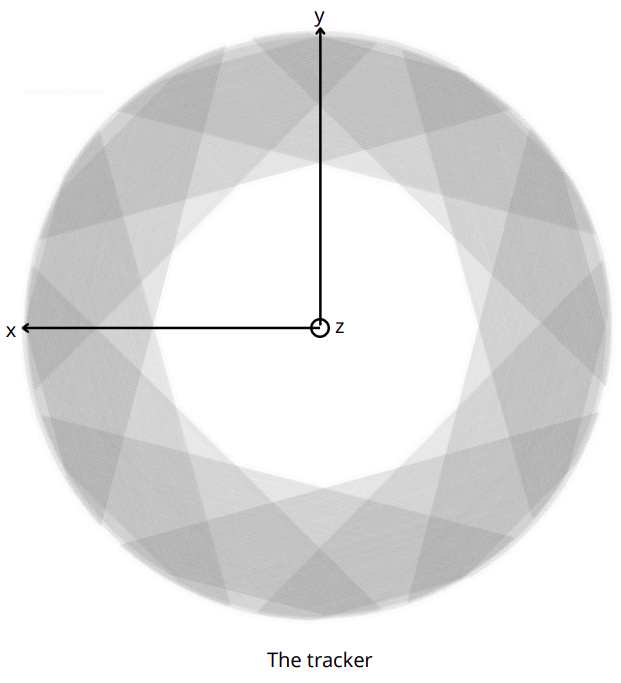
\includegraphics[width =0.5\textwidth]{figures/png/Screenshot_20240526_164527.png}
    \caption[Schematic view of a tracker station and 
    the coordinate system.]{Schematic view of a tracker station 
    and definition of the coordinate system used for the analysis. 
    Different shades of gray indicate different numbers of overlapping panel.}
    \label{fig:coordinate}
\end{figure}
\section{Monte Carlo event selection}\label{eventselection}

Since in the Mu2e simulation the tracker is made of 18 stations, to 
perform this study, we selected those events where a 
cosmic muon crosses the first station.

Although the station has four layers, 
the panel geometry does not provide a uniform
coverage: there are regions of the 
detector where a particle with a trajectory orthogonal
to the panel crosses four, three, two or even only one 
detector layer (Figure \ref{fig:coordinate}). Given the
rotation angles of the panels within the same 
face and between different faces, if this particle
crosses four layers, the straws of the four 
panels are not parallel to each other.
Each straw can be parameterized as a straight line 
lying on a plane $z = z_i$, where $z_i$ is the $z$ 
coordinate of the panel which contains the straw:
\begin{equation}\label{equaretta}
    (D_{x,i}t+M_{x,i},D_{y,i}t+M_{y,i},z_i)
\end{equation}
where $D_{x,i}$, $D_{y,i}$ are the $x$ and $y$ 
$i$-th straws' direction cosines and sines respectively, 
while $M_{x,i}$, $M_{y,i}$ are the $x$, $y$ straws' midpoints.

To perform this study, it is necessary to 
reconstruct the 3D trajectory of the cosmic muon, 
which requires at least two 3D points along the muon's 
trajectory. The $x$ and $y$ coordinates of 
the each required 3D point can be determined 
from the intersection of one pair of straws. Since all straws within a single panel are parallel to 
one another, it is necessary to use at least two straws from 
different panels. The intersection of two straws from 
different panels on the same face lies outside the tracker circle 
(Figure \ref{fig:coordinate}), which is not physically possible. 
Therefore, at least one hit per face is required.

The $z$ coordinate of the 3D intersection is determined as the average of the 
straws' $z$ coordinates. Thus, to avoid selecting 
parallel straws in the same plane, 
the first selection cut 
was to require at least one hit per face. 
This first requirement will be denoted as 
4/4 requirement in the following sections.

Since one particle can hit more than one straw within a panel, 
another selection criterion was to choose events 
with fewer than three hit straws per panel. 
This criterion was selected to minimize errors 
in track reconstruction.
\subsection{Panel illumination pattern}
To achieve precise calibration, the hits should 
be distributed uniformly across the panel.
On the other hand, this is 
not what it is obtained, due to the station geometry
and the selection cuts. 
Figure \ref{fig:illumination} shows the 
resulting hit distribution for panel 0 of
plane 0, which corresponds 
to the panel in 
the upper right part of Figure \ref{fig:coordinate}, 
after applying the selection cuts 
outlined in Section 
\ref{eventselection}. 
This panel was picked as one possible 
example, the 
distributions for all panels in 
both planes are similar, as
shown in Appendix \ref{appendix2}.

\begin{figure}[!h]
    \centering
    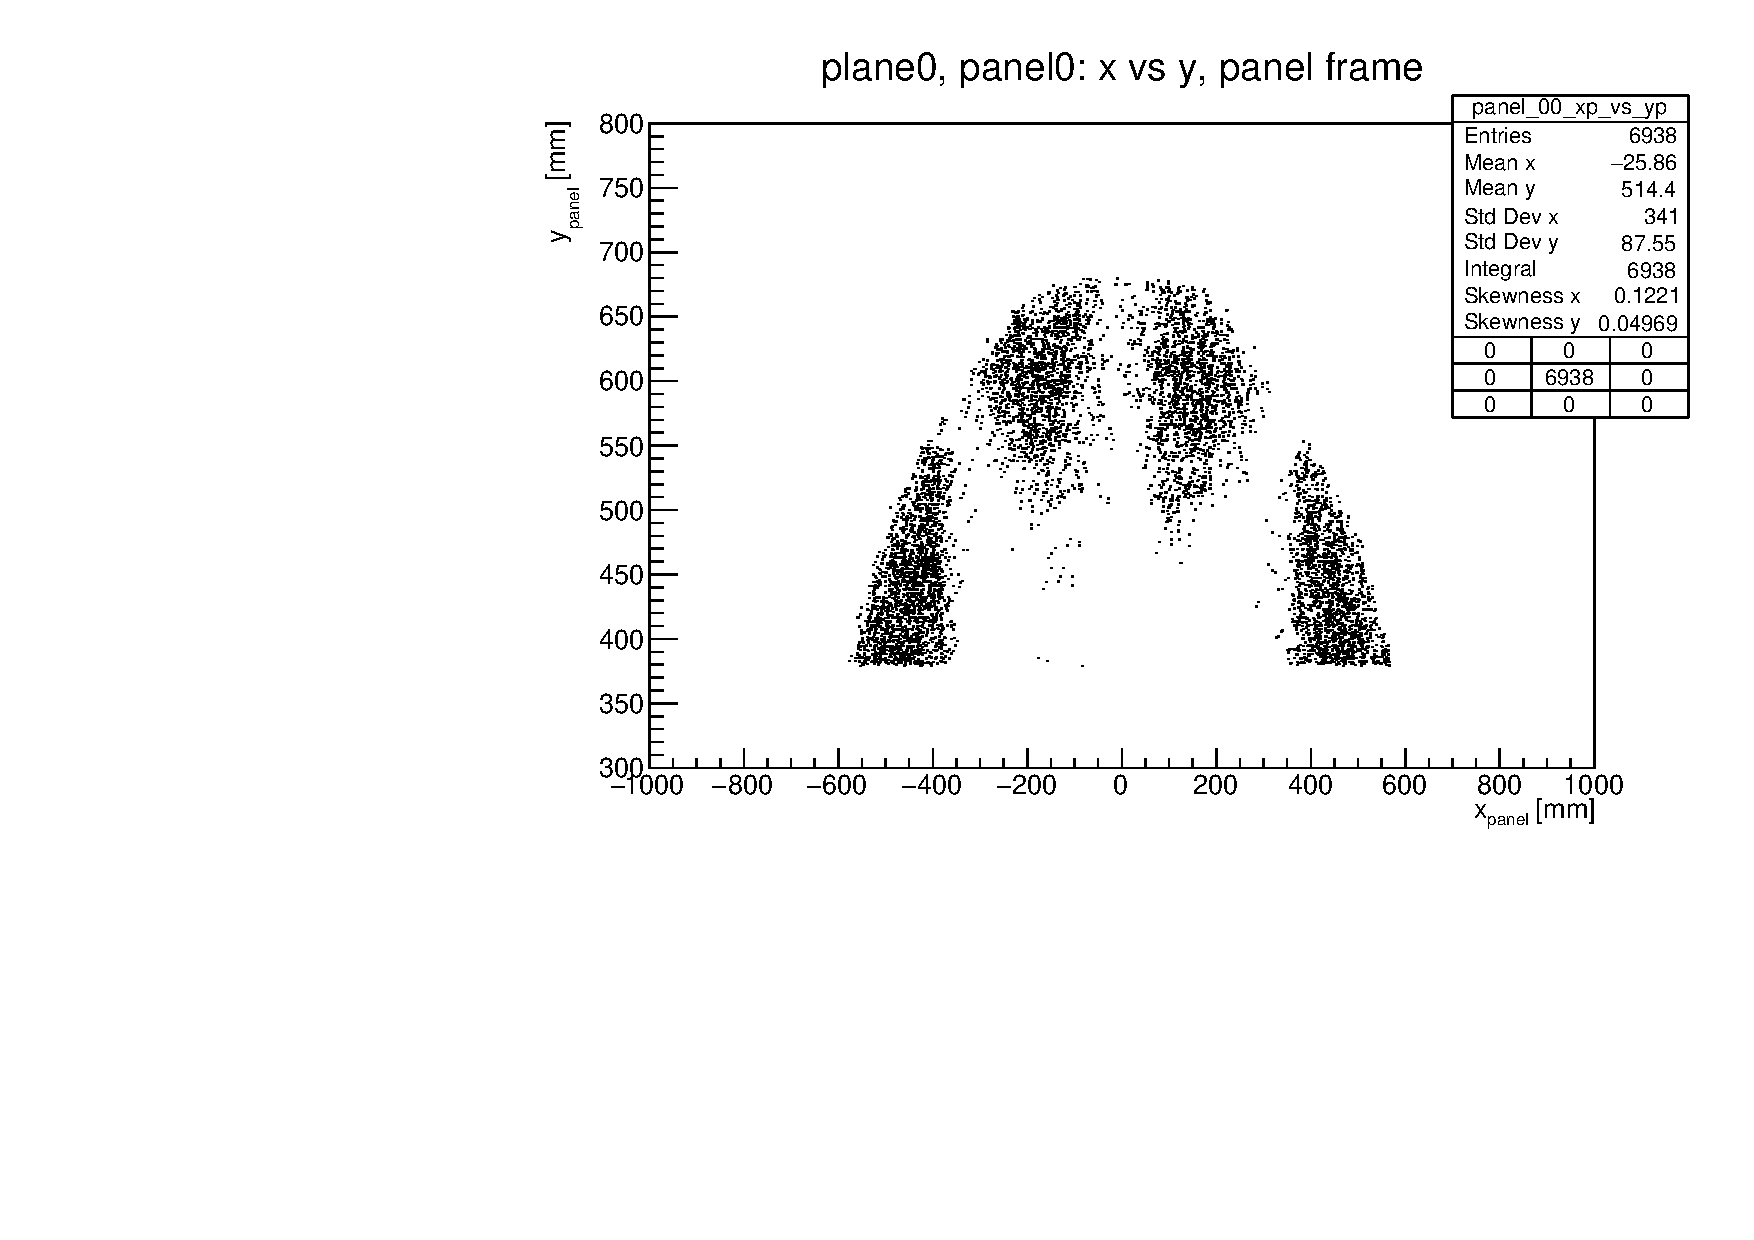
\includegraphics[width =0.8\textwidth]{figures/pdf/xp_vs_yp_panel0.pdf}
    \caption[Monte Carlo illumination across 
    the panel (panel 0, plane 0).]{
        The Monte Carlo illumination 
        across the panel (panel 0, plane 0).
        The selection requires cosmic muons which 
        satisfy the 4/4 requirement and have 
        less than three hits per panel.}
    \label{fig:illumination}
\end{figure}
Figure \ref{fig:illumination} shows a 
non-uniform, or spotty, 
panel illumination. This is due to the 4/4 requirement: 
given the station geometry, the 4/4 overlap 
regions are limited to the edges of the panels (darkest 
areas in Figure \ref{fig:coordinate}). 

Moreover, the 4/4 requirement selects specific
muon directions in the $y$-$z$ plane. 
Figure \ref{fig:myz} shows the 
$m_{yz}=\Delta y /\Delta z$ distribution 
for the selected muons. 
As expected, there are no particles corresponding 
to the $m_{yz}\sim 0$, which corresponds to the  
horizontal direction and 
$m_{yz} \rightarrow \infty$ (vertical), since the 
4/4 requirement is not satisfied by vertical muons. 
The selected muon  
directions tend to have  
$|m_{yz}| \sim 1$, which correspond to  
an angle of approximately 45°.
\begin{figure}[!h]
    \centering
    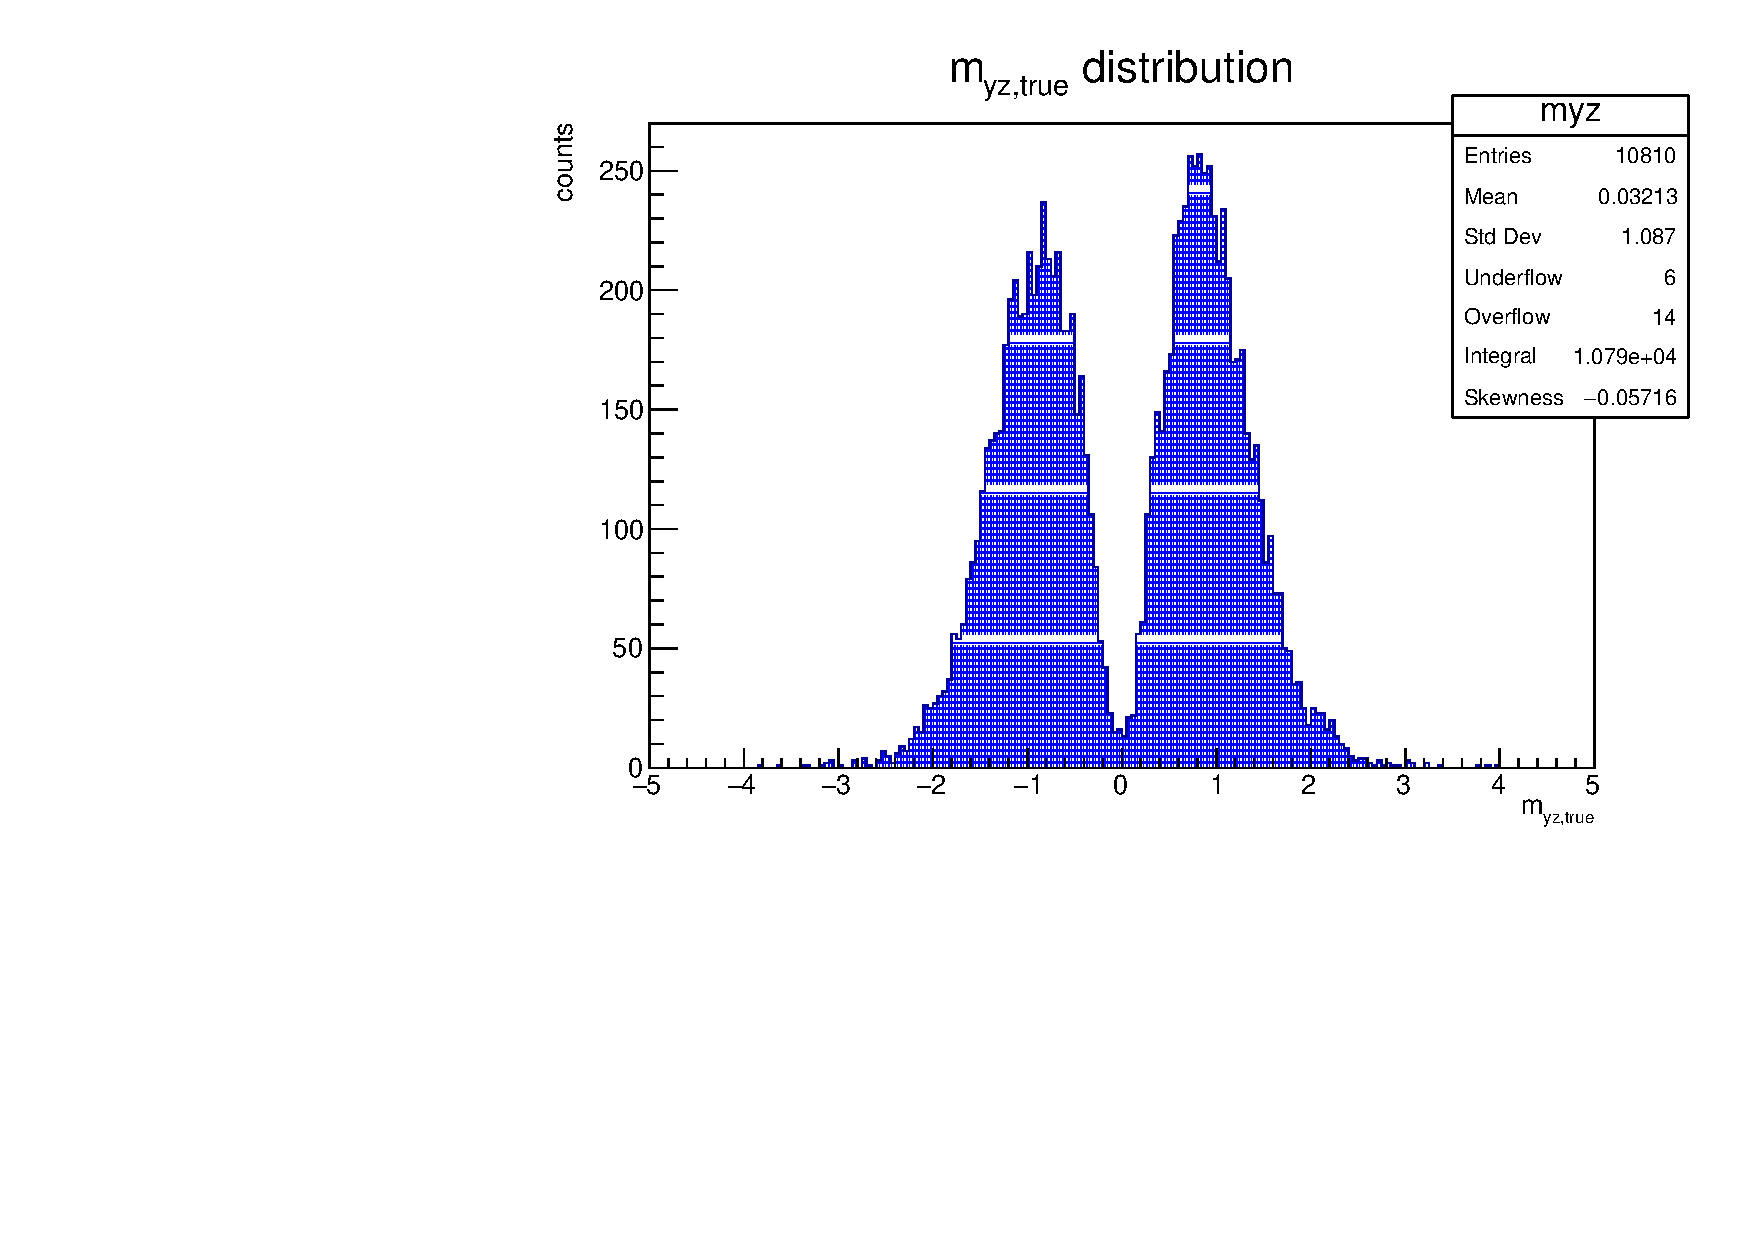
\includegraphics[width =0.8\textwidth]{figures/pdf/myz.pdf}
    \caption[The $y-z$ direction 
    distribution of muons satisfying 4/4 requirement.]{
        $m_{yz}=\Delta y /\Delta z$  
    distribution of muons satisfying 4/4 requirement.}
    \label{fig:myz}
\end{figure}

Figure \ref{fig:illumination} 
shows that there are almost no hits in the central region of the panel. 
This could lead to waveform non-linearities: the signals generated by 
particles at one end of a straw must propagate to the other end as well. 
The leading edge decreases in amplitude and broadens, while moving to 
the other end. This wider portion of the signal contributes the most 
and it may introduce timing systematics.



%Considering a generation plane of an area of  
%$\sim 5$ m$^2$, the resulting rate is $R \sim 380$ Hz. 
%The number of generated events to perform this analysis 
%was $N_{gen}\sim 2\times 10^8$, since the 
%number of cosmics that hit a station is about 2$\times 10^4$, giving a 
%number of hits per panel around 7$\times 10^3$, so 72 hits per straws. 
%But during the calibration, I for sure need more hits per straw, roughly 1000 hits 
%per straw. This gives me a number of generated events of at least 10 times more. 
%Simulating 2$\times 10^9$ cosmic 
%muons on the horizontal plane allows for an 
%approximate estimate of the time necessary to 
%collect a data sample sufficient to perform the 
%calibration, that is
%$T = N_{gen}/R\sim 6$ days, which is 
%excessively long 
%for such a simple calibration. 

%new computation
%integrating the formula -> 77 Hz/m2
%the area of a face (3 panels) is about 0.9 m2
%at this point we need to understand how much we loose considering 
%a vertical station. The most vertical angle one can measure is the arctan of 
%0.7m (radius of the tracker station) divided by 5mm*2*4, that is 4°. 
\section{Reconstructing the muon tracks}\label{reconstruction}
To determine $x_{\text{track}}$ in Equation \ref{ffffff}, 
it is necessary to reconstruct the 3D muon track 
starting from the $StereoHit$ coordinates.
As mentioned relatively to Equation \ref{equaretta}, 
what is known about each single straw is:
\begin{itemize}
    \item the straw direction $(D_{x,i},D_{y,i})$;
    \item the straw midpoint $(M_{x,i},M_{y,i})$;
    \item the straw $z_i$ coordinate.
\end{itemize} 
Track reconstruction begins 
with the sole information of whether 
a straw has been hit or not.
To improve the hit spatial resolution, adjacent 
straws simultaneously hit, which have been most 
likely crossed by the same muon, are combined 
and form the object called $ClusterHit$. 
A maximum of three straws are used to reconstruct a 
$ClusterHit$, to minimize the uncertainty on 
the determination of the 3D intersection points.
This new object represents a 
straw with the same direction and the midpoint 
computed as the average of the midpoints of the straws  
which make it. Since muons with hits in four panels in four different 
faces are selected, four $ClusterHit$s are reconstructed 
within a station. The new $ClusterHit$ 
midpoints will be referred to as 
$(x_{m,i}, y_{m,i}, z_{m,i})$.
Two $ClusterHit$s in the two faces of the same 
plane are combined to determine one $StereoHit$ on 
the $x-y$ plane. 
The $x$ and $y$ coordinates of the 
$StereoHit$ are determined by the 
intersection point of the two 
$ClusterHit$s. The $z$ coordinate of 
the $StereoHit$ is the average of the 
$z$ coordinates of the $ClusterHit$s.
This is reproduced in Figure \ref{fig:stco}.
\begin{figure}[!h]
    \centering
    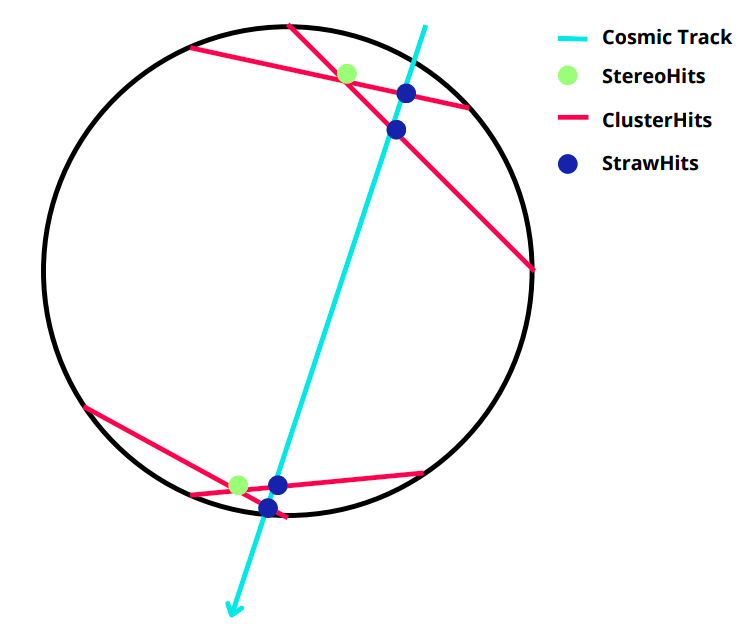
\includegraphics[width =0.6\textwidth]{figures/png/Screenshot_20240810_210144.png}
    \caption[Schematic view of a cosmic muon hitting the vertical 
    oriented station.]{Schematic 
    view of a cosmic muon (light blue) hitting the station 
    (vertical orientation). The red lines are the $ClusterHit$s, 
    the dark blue dots 
    are the $StrawHit$s and the green dots are the $StereoHit$s.}
    \label{fig:stco}
\end{figure}
Considering only one plane and the following 
equations as the $x-y$ $ComboHit$s equations:
\begin{equation}
    \begin{aligned}
        y&=\frac{v_1}{u_1}(x-x_{m,1})+y_{m,1} \\
        y&=\frac{v_2}{u_2}(x-x_{m,2})+y_{m,2} 
    \end{aligned}
    \end{equation}
where $u_i$ is the $ClusterHit$ $x$ direction and $v_i$ is the $ClusterHit$ $y$ direction, the $StereoHit$ coordinates will be:
\begin{equation}\label{x}
    \begin{aligned}
x&=\frac{u_1 u_2(y_{m,1}-y_{m,2}+\frac{v_2}{u_2}x_{m,2}-\frac{v_1}{u_1}x_{m,1})}{v_2 u_1 - v_1 u_2}\\
y&=\frac{v_2}{u_2}\left(\frac{u_1 u_2(y_{m,1}-y_{m,2}+\frac{v_2}{u_2}x_{m,2}-\frac{v_1}{u_1}x_{m,1})}{v_2 u_1 - v_1 u_2}-x_{m,2}\right)+y_{m,2}
\end{aligned}
\end{equation}
In two different planes, there are two $StereoHit$s available, allowing for the reconstruction of the track on $x-y$ and $y-z$ planes. 
Referring to these $StereoHit$s as $(x_1,y_1,z_1)$ and $(x_2,y_2,z_2)$ respectively, the final track slope on $x-y$ plane will be 
denoted as $m_{xy}$, while on the $y-z$ plane it will be denoted as $m_{yz}$. The corresponding $y$-intercepts will be $q_{xy}$ and $q_{yz}$.
The formulas for computing these parameters are as follows:
\begin{equation}
    \begin{aligned}
m_{xy}&=\frac{y_2-y_1}{x_2-x_1}\\
q_{xy}&=-m_{xy} \cdot x_1+y_1
\end{aligned}
\end{equation}
\begin{equation}
    \begin{aligned}
m_{yz}&=\frac{y_2-y_1}{z_2-z_1}\\
q_{yz}&=-m_{yz} \cdot z_1+y_1
\end{aligned}
\end{equation}
To determine the four hit positions of the reconstructed track on the panels, it is necessary to intersect the track with the panels' $z_i$ coordinates. 
The reconstructed hits on the panels will be denoted as $R_{x,i}$ and $R_{y,i}$.
\begin{equation}
    \begin{aligned}
 R_{y,i}&=m_{yz}\cdot z_i+q_{yz}\\
 R_{x,i}&=\frac{(m_{yz}\cdot z_i+q_{yz}-q_{xy})}{m_{xy}}
\end{aligned}
\end{equation}
The bias on the longitudinal position is the difference between 
the reconstructed coordinate and the Monte Carlo position 
on the panel frame.

\section{Results}

This study aims to verify the consistency of the 
calibration procedure with the specified requirements. In particular, since the 
procedure allows to perform an approximate reconstruction 
of the muon track and, thus, of the extrapolated track 
position on the panel, it is necessary to carefully determine 
what is the bias introduced by this procedure,  
to make sure it is well below the threshold of 4 cm.  

Figure \ref{fig:recx} shows the reconstructed 
longitudinal coordinate $x_{\text{track}}$, which is 
determined as the intersection of the reconstructed 
muon track with the mean $z_i$ coordinate of the panel, for panel 0, taken as an example.
Similar patterns were observed for all panels. In this distribution, the bumps 
are a consequence of the 4/4 requirement and overlap of the panels  
being located at the extreme edges. It is also important to observe that 
hits in different regions in $x$ correspond to different 
straws, as can also be seen in Figure \ref{fig:illumination}. 

\begin{figure}[!h]
    \centering
    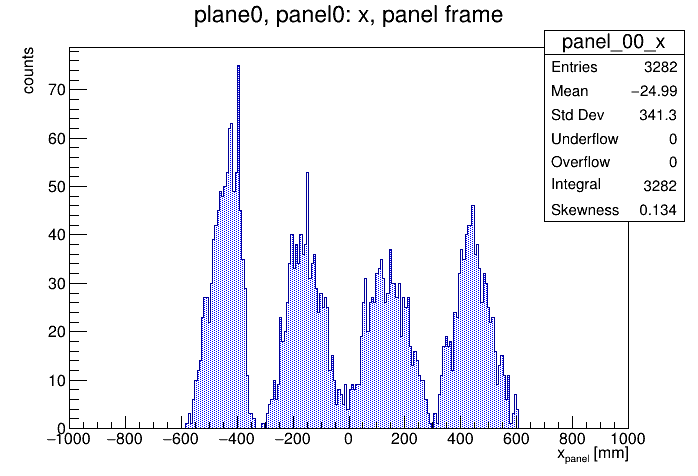
\includegraphics[width=0.8\textwidth]{figures/png/x_panel0.png}
    \caption[The reconstructed longitudinal coordinate in the 0th panel frame.]{The reconstructed longitudinal coordinate in the 0th panel frame.}
    \label{fig:recx}
\end{figure}

Figure \ref{fig:bias} shows the distribution of the longitudinal bias $\Delta x$ determined as the difference between the projection 
of the reconstructed track on the panel and Monte Carlo coordinates. 
The true coordinate is computed as the mean coordinate of the Monte Carlo hits within the panel.
\begin{figure}[!h]
    \centering
    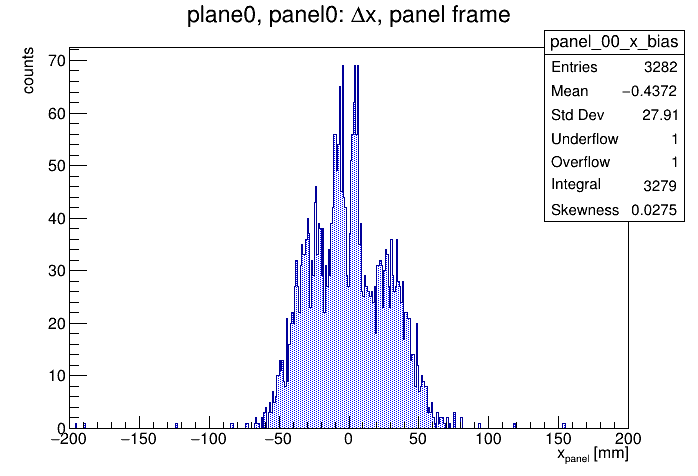
\includegraphics[width=0.8\textwidth]{figures/png/panel_00_x_bias.png}
    \caption[The bias between the reconstructed and the true hit coordinate.]{The longitudinal bias 
    $\Delta x$ between the reconstructed and the true hit coordinate on panel 0. 
    The true coordinate is the mean coordinates of Monte Carlo hits.}
    \label{fig:bias}
\end{figure}
The bias range is approximately [-6,6] cm, indicating a significant systematic factor 
affecting the hit reconstruction. The distribution is similar for all panels. 
One problem is that this distribution is referred to multiple straws, so the 
bias could be very different between straws.

The systematics brought by this type of reconstruction, both for 
the horizontal and vertical orientation, arise from the fact that $m_{yz}=\frac{\Delta y}{\Delta z}$ 
is not accurately reconstructed and the reconstructed coordinates depend on this 
value, as demonstrated in Section \ref{reconstruction}. 
This discrepancy arises when the true hit position, far from the straws midpoint, 
results in incorrectly reconstructed tracks' direction on the $y-z$ plane, leading to the erroneous 
reconstruciton of cosmic muons as horizontal tracks.
\begin{figure}[!h]
    \centering
    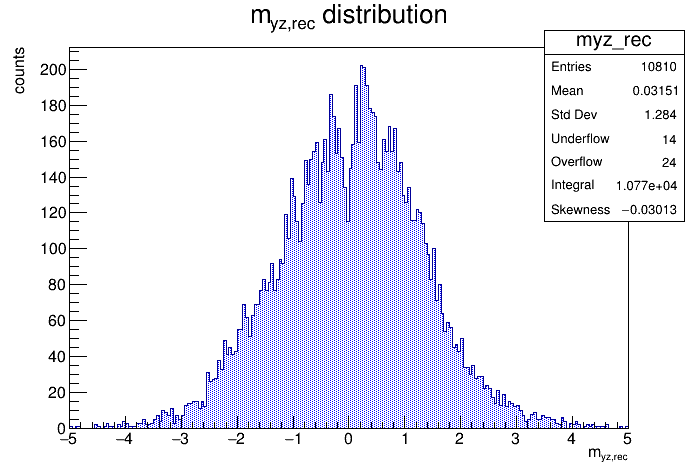
\includegraphics[width=0.8\textwidth]{figures/png/myz_rec.png}
    \caption[The reconstructed $y-z$ direction distribution of cosmic rays.]{The reconstructed $y-z$ direction distribution of cosmic rays ($m_{yz}=\Delta y /\Delta z$).}
    \label{fig:myzrec}
  \end{figure}
Figure \ref{fig:myzrec} reports the reconstructed $m_{yz}$ distribution, which shows 
a significant peak at the value of 0, corresponding to cosmic muons erroneously 
reconstructed as horizontal. 
No horizontal muons are in the sample, as can be seen from Figure \ref{fig:myz}.

The main difference between the horizontal and vertical orientation can be better 
understood looking at Figure \ref{fig:rec2D} and \ref{fig:profile}. 
\begin{figure}[!h]
    \centering
    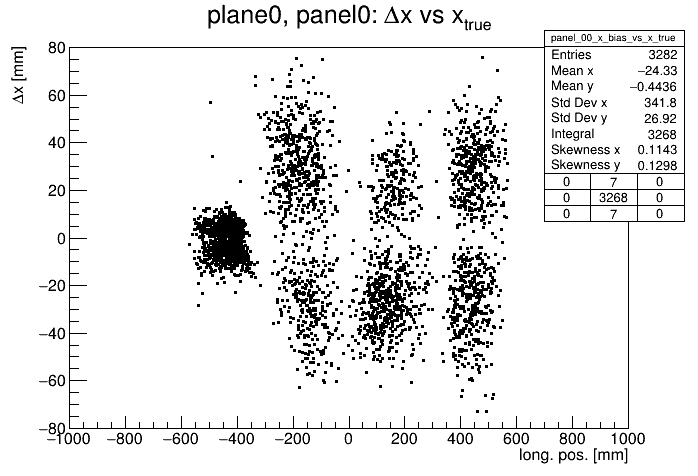
\includegraphics[width=0.8\textwidth]{figures/png/panel_00_x_bias_vs_x.png}
    \caption[The 2D histogram of the longitudinal bias versus the true coordinate.]{The 2D histogram of 
    the longitudinal bias versus the true longitudinal coordinate.}
    \label{fig:rec2D}
\end{figure}
\begin{figure}[!h]
    \centering
    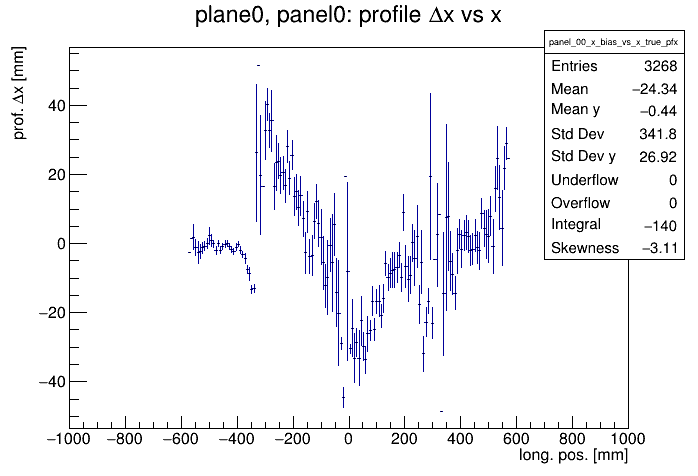
\includegraphics[width=0.8\textwidth]{figures/png/panel_00_x_bias_vs_x_prof.png}
    \caption[The profile of the longitudinal bias versus the true longitudinal coordinate.]{The profile of the longitudinal bias versus the true longitudinal coordinate.}
    \label{fig:profile}
\end{figure}
The first one shows the 2D distribution of $\Delta x$ 
versus the true position and the second one shows the profile histogram of $\Delta x$ versus 
the true coordinates. 
Figure \ref{fig:rec2D}, shows four different 
spots on the $x$ axis corresponding to 
the overlap regions. Each spot refers to 
different straws. The two spots on the $y$ 
axis correspond to cosmics with different orientations. 

To assess the systematic impact on the reconstructed coordinates, it is essential 
to look also at the profile histogram of the bias versus the true coordinates. 
Profile histograms are used to represent the mean value of $y$ and its error for each bin in $x$. 
The default displayed error is the standard error on the mean. 
Figure \ref{fig:profile} reveals a systematic effect in determining the 
longitudinal position within a range exceeding [-4,4] cm. 
This plot suggests that the mean may not be a reliable estimator 
of the bias. The main issue with this plot is that, in the vertical orientation, the stereo 
reconstruction biases for tracks with positive and negative values of 
$m_{yz}$ do not cancel each other out.
Considering the vertical orientation and imagining two cosmic muons  
with opposite $y-z$ orientations, since cosmics come from the top and travel 
downwards, the first particle would hit plane 0 and then plane 1, while the second 
would hit plane 1 first and then plane 0, with all hits occurring on different 
panels. For this reason, opposite $y-z$ orientated cosmics do not appear on the same profile 
histogram for a single panel. In the horizontal case, the same systematics apply as in the vertical case. 
However, in this scenario, both cosmic rays would first hit plane 0 and then 
plane 1, and since most muons have a vertical trajectory, they would hit most likely  
the same panels. Therefore, the mean could serve as a reasonable estimator of the bias in this case.

The narrower spot on the left (CAL side) in Figure \ref{fig:rec2D} and \ref{fig:profile} 
corresponds to the overlap of one panel with another located 
on a different face, oriented at 90° relative to the first one. 
Considering face 0 of the first plane and face 0 of the second plane, 
rotated by 180° about the $y$ axis (the same applies for the other faces), 
there are three pairs of panels whose relative angle is 90° (Figure \ref{fig:coordinate}). 
This type of overlap minimizes the systematic effect and consequently the bias that was explained earlier.

Under these conditions, achieving the required accuracy 
for the calibration is expected to become challenging. 


  
  \section{Conclusions}
  This chapter discusses the initial steps towards the tracker calibration.
  The ultimate goal is to perform a timing calibration of 
  the first assembled station of the tracker using cosmic muons, aiming for a longitudinal hit 
  position resolution better than 4 cm. This requires determining the signal propagation velocity and 
  channel-to-channel delays. The TDCs will measure the signal arrival times, $t_1$ and $t_2$. 
  The calibration will be performed reconstructing the track position along the straw and comparing it with the arrival times. 
  Due to operational constraints of the station, such as gas distribution, fragility, and space, a 
  vertical station calibration was considered to be the best option for our goals.
  The focus of this chapter was on the reconstruction of the trajectories 
  of simulated cosmic muons within a vertically oriented station, as well as the 
  analysis of potential biases and systematic errors that could arise from this particular orientation. 
  I reconstructed $x_{\text{track}}$ using only the information of whether a straw was crossed 
  or not by a cosmic muon, using only the geometry of the tracker station.

This analysis demonstrated that the vertical orientation for calibrating a station is not optimal. This is due to several reasons:
\begin{itemize}
    \item the selection criteria in Section \ref{eventselection} select cosmic muons with orientations that affect panel illumination. 
    The illumination is non-uniform, and moreover, there are almost no hits in the central region of the panel, which could result in waveform non-linearities;
    \item the longitudinal bias $\Delta x$ range is approximately [-6,6] cm, indicating a significant systematic factor 
    affecting the hit reconstruction. The systematics arise from the fact that $m_{yz}$ is not accurately reconstructed.
    In fact, if the true hit position is far from the midpoint of the straws, the reconstructed tracks'
    direction on the $y-z$ plane is completely different from the true one;
    \item the 2D distribution of the $\Delta x$ versus the true position shows 
    four distinct spots on the $x$ axis corresponding to the overlap regions. Each spot refers to different straws. 
    The profile histogram of this distribution reveals a systematic effect in determining the 
    longitudinal position within a range greater than [-4,4] cm. The main issue is that, in the vertical orientation, the stereo 
    reconstruction biases for tracks with positive and negative values of $m_{yz}$ do not cancel each other out.
\end{itemize}

In addition to these results, there is one last factor we need to consider: the rate and the consequent data taking time.
For the vertical orientation, the rate must be scaled by two additional factors compared to the horizontal one.
Considering only muons at 45° (Figure \ref{fig:myz}), the first factor, 
approximately $1/\cos^2\theta \sim 1/2$, accounts for the angular dependence of the flux,
and the second factor, $1/\sqrt{2}$, accounts for cosmic rays striking the station at a 45° angle.
However, estimating the rate is quite complicated. In fact, these are not the main contributors to the difference between the two rates.
With the horizontal orientation, it is possible to reconstruct a particle track without the 4/4 requirement,
instead only requiring that the particle crosses two panels on different faces, as most muons are vertical.
On the other hand, if the vertical orientation is the only possible configuration,
the analysis must account for all the biases in every straw.
Consequently, much more data is required, as the number of parameters in the analysis increases.


Therefore, an alternative orientation or method should be considered to optimize the calibration process and achieve more accurate results.
For this reason, a new mechanical solution to address the problems outlined in Section \ref{gassystem} is currently under development.
%The consequence of the 4/4 requirement is also a 
%significant reduction of the total muon rate. 
%\subsection{Expected muon rate}\label{ratetracker}
%The cosmic muons sample rate can be computed by 
%integrating the flux on the solid angle, on 
%the muon energy described in Section \ref{genplane}:
%\begin{equation}\label{intef}
%   R= \int \frac{\text{d} I}{d E_\mu \text{d} \Omega \text{d} t \text{d} S}orientation \text{d} S_{\perp} \text{d} \Omega \text{d} E_\mu
%    \end{equation}
%where $\text{d}S_\perp= \text{d}S \text{cos}\theta$ 
%is the projection of the surface element on the 
%plane perpendicular to the cosmics flux. 
%The energy and angle ranges selected for this 
%simulation are respectively 0.5 GeV < $E_\mu$ < 500 GeV, 
%which selects muons not absorbed in the 
%concrete layer posed above the tracker, 
%and 0° < $\theta^*$ < 90°. 
%By integrating Eq. \ref{intef}, we obtain a flux of approximately 172 Hz/m$^2$.  
%Given an area of $\sim$0.9 m$^2$, which corresponds to the sensitive area of one face, 
%the rate is about $R\sim$155 Hz in the horizontal configuration.  
%For the vertical station, let us simplify the case by considering only 
%muons at a 45° angle, which are the most probable (Figure \ref{fig:myz}):  

%Therefore, the rate in the vertical case is approximately $R\sim$55 Hz.

%To perform an initial calibration, at least $10^3$ hits per straw are required, 
%which corresponds to a total of $N \sim 2.88 \times 10^5$ cosmics hitting one station. 
%This translates to a calibration time of $T = N/R \sim 30$ minutes per station 
%in the horizontal configuration, and about 1.5 hours for the vertically oriented station.  
%Considering 18 stations, a full day of continuous cosmic ray data acquisition 
%would be required for the entire tracker in the vertical configuration, 
%which is excessively long for such a straightforward calibration. In contrast, 
%only a few hours would be necessary in the horizontal configuration.



